%-------------------------------------------------------------------------------
%   PACKAGES AND OTHER DOCUMENT CONFIGURATIONS
%-------------------------------------------------------------------------------
\documentclass[paper=a4, fontsize=11pt]{scrartcl} % A4 paper and 11pt font size
\usepackage{fancyhdr} % Required for custom headers
\usepackage{lastpage} % Required to determine the last page for the footer
\usepackage{extramarks} % Required for headers and footers
\usepackage[usenames,dvipsnames]{color} % Required for custom colors
\usepackage{graphicx} % Required to insert images
\usepackage{listings} % Required for insertion of code
\usepackage{courier} % Required for the courier font
\usepackage[T1]{fontenc} % Use 8-bit encoding that has 256 glyphs
\usepackage[english]{babel} % English language/hyphenation
\usepackage{amsmath,amsfonts,amsthm} % Math packages
\usepackage{enumitem}
\usepackage{algorithm}
\usepackage{algpseudocode}

\usepackage{sectsty} % Allows customizing section commands
\allsectionsfont{\centering \normalfont\scshape} % Make all sections centered, 
                                                 % the default font and small 
                                                 % caps

\pagestyle{fancyplain} % Makes all pages in the document conform to the custom
                       % headers and footers
\fancyhead{} % No page header - if you want one, create it in the same way as 
             % the footers below
\fancyfoot[L]{} % Empty left footer
\fancyfoot[C]{} % Empty center footer
\fancyfoot[R]{\thepage} % Page numbering for right footer
\renewcommand{\headrulewidth}{0pt} % Remove header underlines
\renewcommand{\footrulewidth}{0pt} % Remove footer underlines
\setlength{\headheight}{13.6pt} % Customize the height of the header

\numberwithin{equation}{section} % Number equations within sections (i.e. 1.1, 
                                 % 1.2, 2.1, 2.2 instead of 1, 2, 3, 4)
\numberwithin{figure}{section} % Number figures within sections (i.e. 1.1, 1.2,
                               % 2.1, 2.2 instead of 1, 2, 3, 4)
\numberwithin{table}{section} % Number tables within sections (i.e. 1.1, 1.2, 
                              % 2.1, 2.2 instead of 1, 2, 3, 4)

\setlength\parindent{0pt} % Removes all indentation from paragraphs - comment 
                          % this line for an assignment with lots of text

%-------------------------------------------------------------------------------
%   TITLE SECTION
%-------------------------------------------------------------------------------

\newcommand{\horrule}[1]{\rule{\linewidth}{#1}} % horizontal cmd, arg = height
\newcommand{\name}{Colin Bradford} % student name
\newcommand{\hwnum}{3} % homework number
\newcommand{\classnum}{CS 325} % class num with abreviation
\newcommand{\classname}{Analysis of Algorithms} % name of class
\newcommand{\hwtitle}{\classnum: Project \hwnum}

\title{ 
    \normalfont \normalsize 
    \textsc{Oregon State University} \\ [25pt]
    \large Project Group 21
    \horrule{0.5pt} \\[0.4cm] % Thin top horizontal rule
    \huge \hwtitle \\ % The assignment title
    \horrule{2pt} \\[0.5cm] % Thick bottom horizontal rule
}

\author{
    Colin Bradford
    \and
    Charles Jenkins
    \and
    Albert Le
} % Your name

\date{\normalsize\today} % Today's date or a custom date

%-------------------------------------------------------------------------------
%   DOCUMENT
%-------------------------------------------------------------------------------
\begin{document}

\maketitle % Print the title

\section{Problem 1}
\textbf{Part A:}

    \textbf{i. Linear Problem Formulation}\newline
    
    Let each route be represented as variables of the form "SourceDestination." For example a route from Plant 1 to Warehouse 1 would be "p1w1."\newline
    

    Objective function:\newline
    
    Minimize:\newline
    
    10 p1w1 + 15 p1w2 + 11 p2w1 + 8 p2w2 + 13 p3w1 + 8 p3w2 + 9 p3w3 
	  + 14 p4w2 + 8 p4w3 + 5 w1r1 + 6 w1r2 + 7 w1r3 + 10 w1r4 + 12 w2r3 
	  + 8 w2r4 + 10 w2r5 + 14 w2r6 + 14 w3r4 + 12 w3r5 + 12 w3r6 + 6 w3r7\newline
	  
	
	Subject To:\newline
		
		Supply Constraints:\newline
		   p1w1 + p1w2 = 150\newline
		   p2w1 + p2w2 = 450\newline
		   p3w1 + p3w2 + p3w3 = 250\newline
		   p4w2 + p4w3 = 150\newline
		
		Demand Constraints:\newline
		   w1r1 = 100\newline
		   w1r2 = 150\newline
		   w1r3 + w2r3 = 100\newline
		   w1r4 + w2r4 + w3r4 = 200\newline
		   w2r5 + w3r5 = 200\newline
		   w2r6 + w3r6 = 150\newline
		   w3r7 = 100\newline
		
		Balancing Constraints:\newline
		   p1w1 + p2w1 + p3w1 - w1r1 - w1r2 - w1r3 - w1r4 <= 0\newline
		   p1w2 + p2w2 + p3w2 + p4w2 - w2r3 - w2r4 - w2r5 - w2r6 <= 0\newline
		   p3w3 + p4w3 - w3r4 - w3r5 - w3r6 - w3r7 <= 0\newline
		
		Non-negativity Constraints:\newline
		   p1w1, p1w2, p2w1, p2w2, p3w1, p3w2, p3w3, p4w2, p4w3, w1r1, w1r2, w1r3, w1r4, w2r3, w2r4, w2r5, w2r6, w3r4, w3r5, w3r6, w3r7 >= 0\newline
    
    \textbf{ii. LINDO Code and Output}
    
    \begin{verbatim}
	MIN 10 p1w1 + 15 p1w2 + 11 p2w1 + 8 p2w2 + 13 p3w1 + 8 p3w2 + 9 p3w3 
	  + 14 p4w2 + 8 p4w3 + 5 w1r1 + 6 w1r2 + 7 w1r3 + 10 w1r4 + 12 w2r3 
	  + 8 w2r4 + 10 w2r5 + 14 w2r6 + 14 w3r4 + 12 w3r5 + 12 w3r6 + 6 w3r7
	ST
		   p1w1 + p1w2 = 150
		   p2w1 + p2w2 = 450
		   p3w1 + p3w2 + p3w3 = 250
		   p4w2 + p4w3 = 150	
		   w1r1 = 100
		   w1r2 = 150
		   w1r3 + w2r3 = 100
		   w1r4 + w2r4 + w3r4 = 200	
		   w2r5 + w3r5 = 200
		   w2r6 + w3r6 = 150
		   w3r7 = 100
		   p1w1 + p2w1 + p3w1 - w1r1 - w1r2 - w1r3 - w1r4 <= 0 
		   p1w2 + p2w2 + p3w2 + p4w2 - w2r3 - w2r4 - w2r5 - w2r6 <= 0
		   p3w3 + p4w3 - w3r4 - w3r5 - w3r6 - w3r7 <= 0 
		   p1w1 > 0
		   p1w2 > 0
		   p2w1 > 0
		   p2w2 > 0
		   p3w1 > 0
		   p3w2 > 0
		   p3w3 > 0
		   p4w2 > 0
		   p4w3 > 0
		   w1r1 > 0
		   w1r2 > 0
		   w1r3 > 0
		   w1r4 > 0
		   w2r3 > 0
		   w2r4 > 0
		   w2r5 > 0
		   w2r6 > 0
		   w3r4 > 0
		   w3r5 > 0
		   w3r6 > 0
		   w3r7 > 0
	END
	
	
 LP OPTIMUM FOUND AT STEP     13

        OBJECTIVE FUNCTION VALUE

        1)      17100.00

  VARIABLE        VALUE          REDUCED COST
      P1W1       150.000000          0.000000
      P1W2         0.000000          8.000000
      P2W1       200.000000          0.000000
      P2W2       250.000000          0.000000
      P3W1         0.000000          2.000000
      P3W2       150.000000          0.000000
      P3W3       100.000000          0.000000
      P4W2         0.000000          7.000000
      P4W3       150.000000          0.000000
      W1R1       100.000000          0.000000
      W1R2       150.000000          0.000000
      W1R3       100.000000          0.000000
      W1R4         0.000000          5.000000
      W2R3         0.000000          2.000000
      W2R4       200.000000          0.000000
      W2R5       200.000000          0.000000
      W2R6         0.000000          1.000000
      W3R4         0.000000          7.000000
      W3R5         0.000000          3.000000
      W3R6       150.000000          0.000000
      W3R7       100.000000          0.000000


       ROW   SLACK OR SURPLUS     DUAL PRICES
        2)         0.000000        -10.000000
        3)         0.000000        -11.000000
        4)         0.000000        -11.000000
        5)         0.000000        -10.000000
        6)         0.000000         -5.000000
        7)         0.000000         -6.000000
        8)         0.000000         -7.000000
        9)         0.000000         -5.000000
       10)         0.000000         -7.000000
       11)         0.000000        -10.000000
       12)         0.000000         -4.000000
       13)         0.000000          0.000000
       14)         0.000000          3.000000
       15)         0.000000          2.000000
       16)       150.000000          0.000000
       17)         0.000000          0.000000
       18)       200.000000          0.000000
       19)       250.000000          0.000000
       20)         0.000000          0.000000
       21)       150.000000          0.000000
       22)       100.000000          0.000000
       23)         0.000000          0.000000
       24)       150.000000          0.000000
       25)       100.000000          0.000000
       26)       150.000000          0.000000
       27)       100.000000          0.000000
       28)         0.000000          0.000000
       29)         0.000000          0.000000
       30)       200.000000          0.000000
       31)       200.000000          0.000000
       32)         0.000000          0.000000
       33)         0.000000          0.000000
       34)         0.000000          0.000000
       35)       150.000000          0.000000
       36)       100.000000          0.000000

 NO. ITERATIONS=      13
    \end{verbatim}
    \textbf{iii. Optimal Shipping Routes and Minimum Cost}\newline
    
    The optimal shipping routes and quantity of refrigerators per route are:
    \begin{verbatim}
	  Route      Refrigerators
      P1W1       150
      P2W1       200
      P2W2       250
      P3W2       150
      P3W3       100
      P4W3       150
      W1R1       100
      W1R2       150
      W1R3       100
      W2R4       200
      W2R5       200
      W3R6       150
      W3R7       100
    \end{verbatim}

	The optimal minimum cost is \$17,100\newline
    
\textbf{Part B:}\newline
	To remove Warehouse 2 and all its associated routes, we remove all variables in our equation that contain "w2" in it. The resulting LINDO code is as follows:

	\begin{verbatim}
	MIN 10 p1w1 + 11 p2w1 + 13 p3w1 + 9 p3w3 + 8 p4w3 + 5 w1r1 + 6 w1r2 
	   + 7 w1r3 + 10 w1r4 + 14 w3r4 + 12 w3r5 + 12 w3r6 + 6 w3r7
	ST
	   p1w1 = 150
	   p2w1 = 450
	   p3w1 + p3w3 = 250
	   p4w3 = 150	
	   w1r1 = 100
	   w1r2 = 150
	   w1r3 = 100
	   w1r4 + w3r4 = 200	
	   w3r5 = 200
	   w3r6 = 150
	   w3r7 = 100
	   p1w1 + p2w1 + p3w1 - w1r1 - w1r2 - w1r3 - w1r4 <= 0 
	   p3w3 + p4w3 - w3r4 - w3r5 - w3r6 - w3r7 <= 0 
	   p1w1 > 0
	   p2w1 > 0
	   p3w1 > 0
	   p3w3 > 0
	   p4w3 > 0
	   w1r1 > 0
	   w1r2 > 0
	   w1r3 > 0
	   w1r4 > 0
	   w3r4 > 0
	   w3r5 > 0
	   w3r6 > 0
	   w3r7 > 0
	END
	\end{verbatim}
	
	Upon execution of the code, we are met with these solution infeasibility notices:\newline
	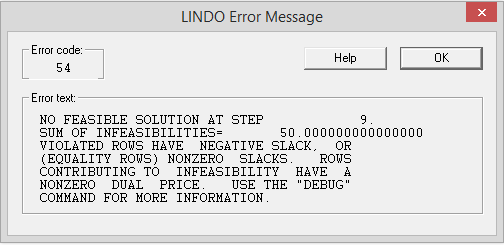
\includegraphics[width=\textwidth]{p1b-err}
	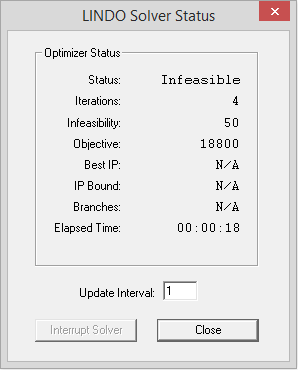
\includegraphics[width=\textwidth]{p1b}
	
	There is no feasible solution here because Warehouse 3's total possible supply (400) is not capable of supporting the combined demand of R4, R5, R6, and R7 (650). On the other hand, Warehouse 1 is in fact capable of supporting R1, R2, R3, and R4 with its 850 supply to 550 demand ratio, but that still does not solve the larger supply chain deficit and feasibility issue. Overall, we need Warehouse 2 to supplement the supply to R3, R4, R5, and R6 and sufficiently "spread the load" on the warehouses.\newline
    
\textbf{Part C:}\newline

To simulate the limitation of 100 shipments (inbound and outbound) on Warehouse 2, we add two new constraints to our code for Part A. The constraints limit the inbound and outbound shipments to being less than or equal to 100.\newline

LINDO Code and Output:
\begin{verbatim}
MIN 10 p1w1 + 15 p1w2 + 11 p2w1 + 8 p2w2 + 13 p3w1 + 8 p3w2 + 9 p3w3 
  + 14 p4w2 + 8 p4w3 + 5 w1r1 + 6 w1r2 + 7 w1r3 + 10 w1r4 + 12 w2r3 
  + 8 w2r4 + 10 w2r5 + 14 w2r6 + 14 w3r4 + 12 w3r5 + 12 w3r6 + 6 w3r7
ST
	   p1w1 + p1w2 = 150
	   p2w1 + p2w2 = 450
	   p3w1 + p3w2 + p3w3 = 250
	   p4w2 + p4w3 = 150	
	   w1r1 = 100
	   w1r2 = 150
	   w1r3 + w2r3 = 100
	   w1r4 + w2r4 + w3r4 = 200	
	   w2r5 + w3r5 = 200
	   w2r6 + w3r6 = 150
	   w3r7 = 100
	   p1w1 + p2w1 + p3w1 - w1r1 - w1r2 - w1r3 - w1r4 <= 0 
	   p1w2 + p2w2 + p3w2 + p4w2 - w2r3 - w2r4 - w2r5 - w2r6 <= 0
	   p3w3 + p4w3 - w3r4 - w3r5 - w3r6 - w3r7 <= 0 
	   p1w1 > 0
	   p1w2 > 0
	   p2w1 > 0
	   p2w2 > 0
	   p3w1 > 0
	   p3w2 > 0
	   p3w3 > 0
	   p4w2 > 0
	   p4w3 > 0
	   w1r1 > 0
	   w1r2 > 0
	   w1r3 > 0
	   w1r4 > 0
	   w2r3 > 0
	   w2r4 > 0
	   w2r5 > 0
	   w2r6 > 0
	   w3r4 > 0
	   w3r5 > 0
	   w3r6 > 0
	   w3r7 > 0
	   p1w2 + p2w2 + p3w2 + p4w2 <= 100
	   w2r3 + w2r4 + w2r5 + w2r6 <= 100
END


 LP OPTIMUM FOUND AT STEP      7

        OBJECTIVE FUNCTION VALUE

        1)      18300.00

  VARIABLE        VALUE          REDUCED COST
      P1W1       150.000000          0.000000
      P1W2         0.000000          8.000000
      P2W1       350.000000          0.000000
      P2W2       100.000000          0.000000
      P3W1         0.000000          4.000000
      P3W2         0.000000          2.000000
      P3W3       250.000000          0.000000
      P4W2         0.000000          9.000000
      P4W3       150.000000          0.000000
      W1R1       100.000000          0.000000
      W1R2       150.000000          0.000000
      W1R3       100.000000          0.000000
      W1R4       150.000000          0.000000
      W2R3         0.000000          7.000000
      W2R4        50.000000          0.000000
      W2R5        50.000000          0.000000
      W2R6         0.000000          4.000000
      W3R4         0.000000          4.000000
      W3R5       150.000000          0.000000
      W3R6       150.000000          0.000000
      W3R7       100.000000          0.000000


       ROW   SLACK OR SURPLUS     DUAL PRICES
        2)         0.000000        -20.000000
        3)         0.000000        -21.000000
        4)         0.000000        -19.000000
        5)         0.000000        -18.000000
        6)         0.000000          5.000000
        7)         0.000000          4.000000
        8)         0.000000          3.000000
        9)         0.000000          0.000000
       10)         0.000000         -2.000000
       11)         0.000000         -2.000000
       12)         0.000000          4.000000
       13)         0.000000         10.000000
       14)         0.000000         13.000000
       15)         0.000000         10.000000
       16)       150.000000          0.000000
       17)         0.000000          0.000000
       18)       350.000000          0.000000
       19)       100.000000          0.000000
       20)         0.000000          0.000000
       21)         0.000000          0.000000
       22)       250.000000          0.000000
       23)         0.000000          0.000000
       24)       150.000000          0.000000
       25)       100.000000          0.000000
       26)       150.000000          0.000000
       27)       100.000000          0.000000
       28)       150.000000          0.000000
       29)         0.000000          0.000000
       30)        50.000000          0.000000
       31)        50.000000          0.000000
       32)         0.000000          0.000000
       33)         0.000000          0.000000
       34)       150.000000          0.000000
       35)       150.000000          0.000000
       36)       100.000000          0.000000
       37)         0.000000          0.000000
       38)         0.000000          5.000000

 NO. ITERATIONS=       7
\end{verbatim}

We see that this is a feasible solution, though it raises our optimal cost from \$17,100 to \$18,300.

The optimal shipping routes and quantity of refrigerators per route are:
    \begin{verbatim}
	  Route      Refrigerators
      P1W1       150
      P2W1       350
      P2W2       100
      P3W3       250
      P4W3       150
      W1R1       100
      W1R2       150
      W1R3       100
      W1R4       150
      W2R4        50
      W2R5        50
      W3R5       150
      W3R6       150
      W3R7       100
    \end{verbatim}
\textbf{Part D:}\newline
For some cost $c_{ab}$ and some route $x_{ab}$ where their subscripts represent the route from a to b, the objective function is:\newline
$Min (\sum_{p}{ \sum_{w}{c_{pw} x_{pw}}} + \sum_{w}{ \sum_{r}{c_{wr} x_{wr}}})$\newline

$s.t.$\newline
(Supply Constraint) For each source node p, where s is supply: $\sum_{w}{x_{pw}} = s_{p}$\newline
(Demand Constraint) For each destination node r, where d is demand: $\sum_{w}{x_{wr}} = d_{r}$\newline
(Balancing Constraint) For each intermediate node w: $\sum_{p}{x_{pw}} - \sum_{r}{x_{wr}} <= 0$\newline
(Non-negativity Constraint) For all nodes p and r: $x_{pw}, x_{wr} >= 0$\newline


\section{Problem 2}
\textbf{Part A:}
	
	\textbf{i. Linear Problem Formulation}\newline
    
    Let each ingredient be represented as variables using the first two letters of the ingredient's name. For example spinach is "sp."\newline
    

    Objective function:\newline
    
    Minimize:\newline
    
    21 to + 16 le + 40 sp + 41 ca + 41 su + 120 sm + 164 ch + 884 oi\newline
	  
	Subject To:\newline
		
		Nutrition Constraints:\newline
		   0.85 to + 1.62 le + 2.86 sp + 0.93 ca + 23.4 su + 16 sm + 9 ch >= 15\newline
		   0.33 to + 0.20 le + 0.39 sp + 0.24 ca + 48.7 su + 5 sm + 2.6 ch + 100 oi >= 2\newline
		   0.33 to + 0.20 le + 0.39 sp + 0.24 ca + 48.7 su + 5 sm + 2.6 ch + 100 oi <= 8\newline
		   4.64 to + 2.37 le + 3.63 sp + 9.58 ca + 15 su + 3 sm + 27 ch >= 4\newline
		   9 to + 28 le + 65 sp + 69 ca + 3.8 su + 120 sm + 78 ch <= 200\newline
		   le + sp - .4le - .4sp - .4to - .4ca - .4su - .4sm - .4ch - .4oi >= 0\newline
		
		Non-negativity Constraints:\newline
		   le, sp, to, ca, su, sm, ch, oi >= 0\newline
    
    \textbf{ii. LINDO Code and Output}
    \begin{verbatim}
MIN 21 to + 16 le + 40 sp + 41 ca + 41 su + 120 sm + 164 ch + 884 oi
ST
   0.85 to + 1.62 le + 2.86 sp + 0.93 ca + 23.4 su + 16 sm + 9 ch >= 15
   0.33 to + 0.20 le + 0.39 sp + 0.24 ca + 48.7 su + 5 sm + 2.6 ch + 100 oi >= 2
   0.33 to + 0.20 le + 0.39 sp + 0.24 ca + 48.7 su + 5 sm + 2.6 ch + 100 oi <= 8
   4.64 to + 2.37 le + 3.63 sp + 9.58 ca + 15 su + 3 sm + 27 ch >= 4
   9 to + 28 le + 65 sp + 69 ca + 3.8 su + 120 sm + 78 ch <= 200
   le + sp - .4le - .4sp - .4to - .4ca - .4su - .4sm - .4ch - .4oi >= 0
   le > 0
   sp > 0
   to > 0
   ca > 0
   su > 0
   sm > 0
   ch > 0
   oi > 0
END

 LP OPTIMUM FOUND AT STEP      8

        OBJECTIVE FUNCTION VALUE

        1)      103.3371

  VARIABLE        VALUE          REDUCED COST
        TO         0.000000         16.520000
        LE         0.561163          0.000000
        SP         0.000000         13.916369
        CA         0.000000         35.535095
        SU         0.084189          0.000000
        SM         0.757556          0.000000
        CH         0.000000         96.583527
        OI         0.000000       1212.744385


       ROW   SLACK OR SURPLUS     DUAL PRICES
        2)         0.000000         -8.632957
        3)         6.000000          0.000000
        4)         0.000000          3.269654
        5)         0.865455          0.000000
        6)        93.060745          0.000000
        7)         0.000000         -4.447570
        8)         0.561163          0.000000
        9)         0.000000          0.000000
       10)         0.000000          0.000000
       11)         0.000000          0.000000
       12)         0.084189          0.000000
       13)         0.757556          0.000000
       14)         0.000000          0.000000
       15)         0.000000          0.000000

 NO. ITERATIONS=       8
    \end{verbatim}
    
    The minimum amount of calories a salad can contain while meeting the nutrition constraints is 103.3371 calories.

The optimal ingredient mix is:
    \begin{verbatim}
	  Ingredient   Amount
        LE         0.561163
        SU         0.084189
        SM         0.757556
    \end{verbatim}
    
    \textbf{iii.}
    The cost of this salad is: $0.561163 * .75 + 0.084189 * .45  + 0.757556 * 2.15 = \$2.0875 \approx \$2.09$
    
\textbf{Part B:}
    
    \textbf{i.}
    
    \textbf{ii.}
    
    \textbf{iii.}
    
\textbf{Part C:}
	
    \textbf{i.}
    
    \textbf{ii.}
    
    \textbf{iii.}
    
\section{Problem 3}
\textbf{Part A:}

    \textbf{i. General Problem Statement}\newline
	Objective:\newline    
    $Min \sum_{i=1}^{n}{b_i}$, for some $b_i$ representing $|y_i - (a_1x_i + a_0)|$ for each i = 1...n\newline
    s.t.\newline
    For each i = 1...n, $b_i - (y_i - (a_1x_i + a_0)) >= 0$\newline
    For each i = 1...n, $b_i + (y_i - (a_1x_i + a_0)) >= 0$\newline
    
    \textbf{ii. LINDO Code and Output}\newline
    \begin{verbatim}
MIN b1 + b2 + b3 + b4 + b5 + b6 + b7
ST
	   b1 + 1 a1 + a0 >= 5
	   b1 - 1 a1 - a0 >= -5
	   b2 + 1 a1 + a0 >= 3
	   b2 - 1 a1 - a0 >= -3
	   b3 + 2 a1 + a0 >= 13
	   b3 - 2 a1 - a0 >= -13
	   b4 + 3 a1 + a0 >= 8
	   b4 - 3 a1 - a0 >= -8
	   b5 + 4 a1 + a0 >= 10
	   b5 - 4 a1 - a0 >= -10
	   b6 + 5 a1 + a0 >= 14
	   b6 - 5 a1 - a0 >= -14
	   b7 + 6 a1 + a0 >= 18
	   b7 - 6 a1 - a0 >= -18
	   b1 > 0
	   b2 > 0
	   b3 > 0
	   b4 > 0
	   b5 > 0
	   b6 > 0
	   b7 > 0
END

 LP OPTIMUM FOUND AT STEP      7

        OBJECTIVE FUNCTION VALUE

        1)      12.25000

  VARIABLE        VALUE          REDUCED COST
        B1         2.000000          0.000000
        B2         0.000000          0.250000
        B3         7.250000          0.000000
        B4         0.500000          0.000000
        B5         1.250000          0.000000
        B6         0.000000          0.750000
        B7         1.250000          0.000000
        A1         2.750000          0.000000
        A0         0.250000          0.000000


       ROW   SLACK OR SURPLUS     DUAL PRICES
        2)         0.000000         -1.000000
        3)         4.000000          0.000000
        4)         0.000000          0.000000
        5)         0.000000         -0.750000
        6)         0.000000         -1.000000
        7)        14.500000          0.000000
        8)         1.000000          0.000000
        9)         0.000000         -1.000000
       10)         2.500000          0.000000
       11)         0.000000         -1.000000
       12)         0.000000          0.000000
       13)         0.000000         -0.250000
       14)         0.000000         -1.000000
       15)         2.500000          0.000000
       16)         2.000000          0.000000
       17)         0.000000          0.000000
       18)         7.250000          0.000000
       19)         0.500000          0.000000
       20)         1.250000          0.000000
       21)         0.000000          0.000000
       22)         1.250000          0.000000

 NO. ITERATIONS=       7
    \end{verbatim}
    
    The sum of the absolute deviations was 12.25.\newline
    
    \textbf{iii. Graph}\newline
    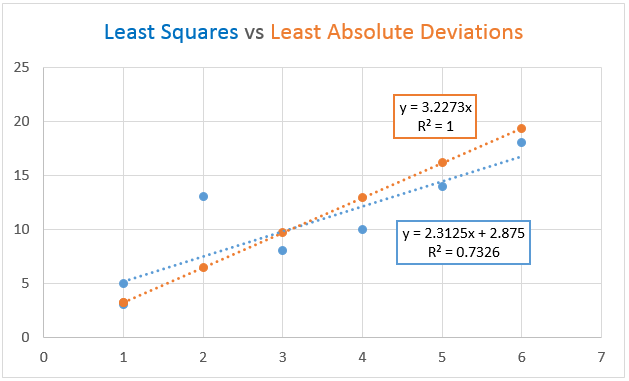
\includegraphics[width=\textwidth]{p3paiii}
    The LAD approach creates a line that has a steeper slope and lesser y-intercept than the least squares line. The line more tightly follows the path of the majority of the data points and seems to be less affected by the outlier at x = 2.\newline
    
\textbf{Part B:}
    
    \textbf{i. General Problem Statement}\newline
    Objective:\newline    
    $Min$ b, for some b representing $Max |y_i - (a_1x_i + a_0)|$\newline
    s.t.\newline
    For each i = 1...n, $b + a_1x_i + a_0 >= y_i$\newline
    For each i = 1...n, $b - a_1x_i - a_0 >= -y_i$\newline
    
    \textbf{ii. LINDO Code and Output}\newline
    \begin{verbatim}
MIN b
ST
	   b + 1 a1 + a0 >= 5
	   b - 1 a1 - a0 >= -5
	   b + 1 a1 + a0 >= 3
	   b - 1 a1 - a0 >= -3
	   b + 2 a1 + a0 >= 13
	   b - 2 a1 - a0 >= -13
	   b + 3 a1 + a0 >= 8
	   b - 3 a1 - a0 >= -8
	   b + 4 a1 + a0 >= 10
	   b - 4 a1 - a0 >= -10
	   b + 5 a1 + a0 >= 14
	   b - 5 a1 - a0 >= -14
	   b + 6 a1 + a0 >= 18
	   b - 6 a1 - a0 >= -18
	   b > 0
END

 LP OPTIMUM FOUND AT STEP      3

        OBJECTIVE FUNCTION VALUE

        1)      3.833333

  VARIABLE        VALUE          REDUCED COST
         B         3.833333          0.000000
        A1         2.333333          0.000000
        A0         4.500000          0.000000


       ROW   SLACK OR SURPLUS     DUAL PRICES
        2)         5.666667          0.000000
        3)         2.000000          0.000000
        4)         7.666667          0.000000
        5)         0.000000         -0.333333
        6)         0.000000         -0.500000
        7)         7.666667          0.000000
        8)         7.333333          0.000000
        9)         0.333333          0.000000
       10)         7.666667          0.000000
       11)         0.000000         -0.166667
       12)         6.000000          0.000000
       13)         1.666667          0.000000
       14)         4.333333          0.000000
       15)         3.333333          0.000000
       16)         3.833333          0.000000

 NO. ITERATIONS=       3
    \end{verbatim}
    
    The min of the max absolute deviations was 3.833333.\newline
    
    \textbf{iii. Graph}\newline
    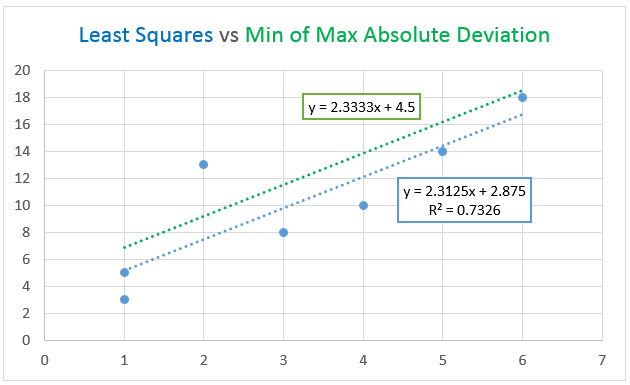
\includegraphics[width=\textwidth]{p3pbiii}
    The MMAD approach gives a line that appears to be more affected by the outlier at x = 2 with a much higher y-intercept than the LAD and least squares approaches. It's slope however, is only slightly steeper than the least squares line. \newline
    
    \textbf{iv. Same Line Data Set}\newline
    Yes, the data set (x,y) = [(1,2), (2,4), (3,6)] computes the same line for all three methods.\newline
    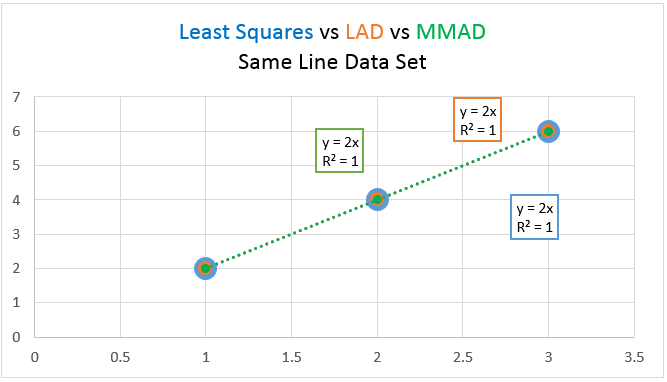
\includegraphics[width=\textwidth]{p3pbiv}
    \begin{verbatim}
LAD Method:    
    
MIN b1 + b2 + b3
ST
	   b1 + 1 a1 + a0 >= 2
	   b1 - 1 a1 - a0 >= -2
	   b2 + 2 a1 + a0 >= 4
	   b2 - 2 a1 - a0 >= -4
	   b3 + 3 a1 + a0 >= 6
	   b3 - 3 a1 - a0 >= -6
	   b1 > 0
	   b2 > 0
	   b3 > 0
END

 LP OPTIMUM FOUND AT STEP      1

        OBJECTIVE FUNCTION VALUE

        1)     0.0000000E+00

  VARIABLE        VALUE          REDUCED COST
        B1         0.000000          1.000000
        B2         0.000000          1.000000
        B3         0.000000          1.000000
        A1         2.000000          0.000000
        A0         0.000000          0.000000


       ROW   SLACK OR SURPLUS     DUAL PRICES
        2)         0.000000          0.000000
        3)         0.000000          0.000000
        4)         0.000000          0.000000
        5)         0.000000          0.000000
        6)         0.000000          0.000000
        7)         0.000000          0.000000
        8)         0.000000          0.000000
        9)         0.000000          0.000000
       10)         0.000000          0.000000

 NO. ITERATIONS=       1
 
MMAD Method:

MIN b
ST
	   b + 1 a1 + a0 >= 2
	   b - 1 a1 - a0 >= -2
	   b + 2 a1 + a0 >= 4
	   b - 2 a1 - a0 >= -4
	   b + 3 a1 + a0 >= 6
	   b - 3 a1 - a0 >= -6
	   b > 0
END

 LP OPTIMUM FOUND AT STEP      1

        OBJECTIVE FUNCTION VALUE

        1)     0.0000000E+00

  VARIABLE        VALUE          REDUCED COST
         B         0.000000          1.000000
        A1         2.000000          0.000000
        A0         0.000000          0.000000


       ROW   SLACK OR SURPLUS     DUAL PRICES
        2)         0.000000          0.000000
        3)         0.000000          0.000000
        4)         0.000000          0.000000
        5)         0.000000          0.000000
        6)         0.000000          0.000000
        7)         0.000000          0.000000
        8)         0.000000          0.000000

 NO. ITERATIONS=       1

Least Squares Line was produced in Excel (see graph above) rather than LINDO.

    \end{verbatim}
    
\textbf{Part C:}
	Objective:\newline    
    $Min \sum_{i=1}^{n}{b_i}$, for some $b_i$ representing $|y_i - (a_2 x_{2i} + a_1x_{1i} + a_0)|$ for each i = 1...n\newline
    s.t.\newline
    For each i = 1...n, $b_i - (y_i - (a_2 x_{2i} + a_1x_{1i} + a_0)) >= 0$\newline
    For each i = 1...n, $b_i + (y_i - (a_2 x_{2i} + a_1x_{1i} + a_0)) >= 0$\newline
	
\begin{verbatim}
MIN b1 + b2 + b3 + b4 + b5 + b6
ST
	   b1 + 1 a2 + 1 a1 + a0  >= 5
	   b1 - 1 a2 - 1 a1 - a0 >= -5
	   b2 + 2 a2 + 1 a1 + a0  >= 9
	   b2 - 2 a2 - 1 a1 - a0 >= -9	
	   b3 + 2 a2 + 2 a1 + a0  >= 12
	   b3 - 2 a2 - 2 a1 - a0 >= -12
	   b4 + 1 a2 + 0 a1 + a0  >= 3
	   b4 - 1 a2 - 0 a1 - a0 >= -3
	   b5 + 0 a2 + 0 a1 + a0  >= 0
	   b5 - 0 a2 - 0 a1 - a0 >= 0
	   b6 + 3 a2 + 1 a1 + a0  >= 11
	   b6 - 3 a2 - 1 a1 - a0 >= -11
	   b1 > 0
	   b2 > 0
	   b3 > 0
	   b4 > 0
	   b5 > 0
	   b6 > 0
END

 LP OPTIMUM FOUND AT STEP      8

        OBJECTIVE FUNCTION VALUE

        1)      2.000000

  VARIABLE        VALUE          REDUCED COST
        B1         1.000000          0.000000
        B2         0.000000          0.000000
        B3         0.000000          0.500000
        B4         0.000000          0.000000
        B5         0.000000          0.500000
        B6         1.000000          0.000000
        A2         3.000000          0.000000
        A1         3.000000          0.000000
        A0         0.000000          0.000000


       ROW   SLACK OR SURPLUS     DUAL PRICES
        2)         2.000000          0.000000
        3)         0.000000         -1.000000
        4)         0.000000         -1.000000
        5)         0.000000          0.000000
        6)         0.000000         -0.500000
        7)         0.000000          0.000000
        8)         0.000000         -1.000000
        9)         0.000000          0.000000
       10)         0.000000          0.000000
       11)         0.000000         -0.500000
       12)         2.000000          0.000000
       13)         0.000000         -1.000000
       14)         1.000000          0.000000
       15)         0.000000          0.000000
       16)         0.000000          0.000000
       17)         0.000000          0.000000
       18)         0.000000          0.000000
       19)         1.000000          0.000000

 NO. ITERATIONS=       8
    \end{verbatim}
    The sum of the absolute deviations was 2.\newline
    The regression model is: $y = 3x_2 + 3x_1 + 0$

\end{document}
%-------------------------------------------------------------------------------


